% carried from the v2 tree (results.tex); the exactness wording and the 8.8 tick were corrected in v3.
\begin{figure*}[tp]\centering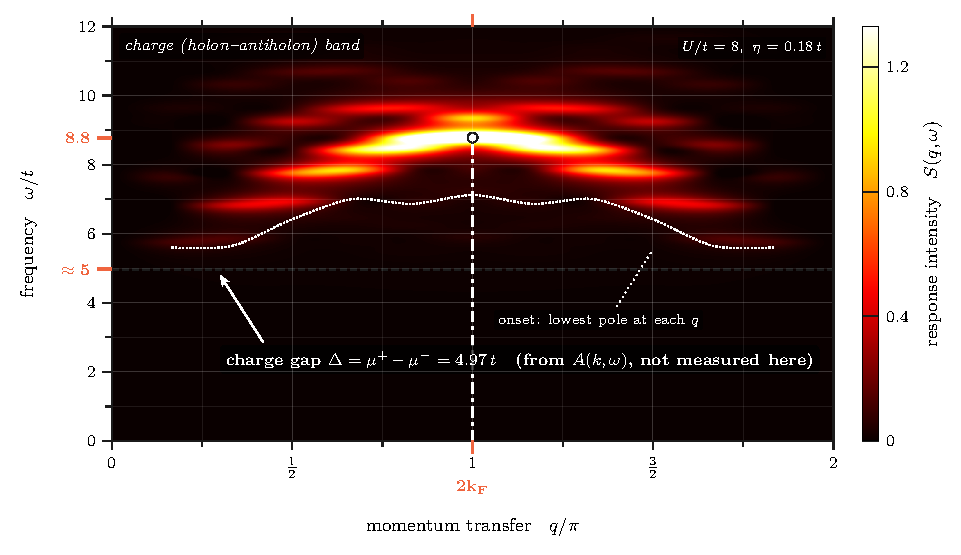
\includegraphics[width=0.92\linewidth]{figs/fig_sqw.pdf}
\caption{\textbf{Dynamical structure factor: the density response.} $S(q,\omega)$ of the
half-filled Hubbard chain ($U/t=8$, $L=12$, Lorentzian broadening $\eta=0.18\,t$)---the density--density
response, a number-conserving (neutral) excitation, computed by a Haydock continued fraction of
depth $n_\ell=150$ in the $N$-particle sector---a finite-depth quadrature of the spectral measure,
not the Lehmann sum (Sec.~\ref{sm:physics}). Colour is the \emph{response intensity} $S(q,\omega)$ (units $1/t$): bright
means the system responds strongly at that $(q,\omega)$, dark means it does not. The weight forms the
two-particle charge (holon--antiholon) band, whose dotted curve is the onset, the lowest pole resolved at each $q$, and sets the
low-frequency scale of the band and traces its lower-boundary dispersion; the diffuse upper
boundary is left unmarked. At $L=12$ this band is six to nine discrete poles per momentum merged by
the broadening, not a dense spectrum (Table~\ref{tab:poles}). Two features are decisive. \emph{(i)}
The band is gapped on the scale of the charge gap: every resolved pole lies above
$\Delta=\mu^{+}-\mu^{-}=4.97\,t$ (exact $(N{\pm}1)$ ground-state energies), the lowest onset
reached here being $5.60\,t$ at $q/\pi=1/6$. The limit $q\to0$ is inaccessible to this observable,
$S(q{=}0,\omega{>}0)$ vanishing identically by density conservation, so $\Delta$ is drawn as a
horizontal reference level imported from the single-particle channel and nothing is claimed about
that limit. It is the \emph{same} Mott gap that
separates the Hubbard bands in the single-particle channel (Fig.~\ref{fig:lattice}): two independent
dynamical observables, one correlation gap. \emph{(ii)} The band peaks at $q=2k_F=\pi$ at
$\omega=8.78\,t$ (coral tick, at the measured peak), within $10\%$ of the bare Hubbard scale
$U=8\,t$ of a doubly-occupied site; the tick marks the peak, not $U$. The reflection
$S(q)=S(2\pi{-}q)$ holds to $\sim\!10^{-4}$ (Lanczos precision), and the analytic f-sum rule
$\int\omega\,S(q,\omega)\,d\omega\propto(1-\cos q)$ is recovered by the plotted (finite-window) grid to
$\sim\!0.3\%$. This is the collective observable the same bitstring-sampled primitive targets; as for
$A(k,\omega)$, faithfully sampling the \emph{full} response carries the sector-fraction cost of
Sec.~\ref{sec:prices}. This channel carries no shot budget: it is a full-sector reference
(Table~\ref{tab:provenance}).}\label{fig:sqw}\end{figure*}
